\section{Potential participants}
\label{sec:part}

% \begin{wrapfigure}{!h}{3.2in}
\begin{figure}[!b]
  \vspace{-0.5cm}
  \centering 
  \subfigure[]{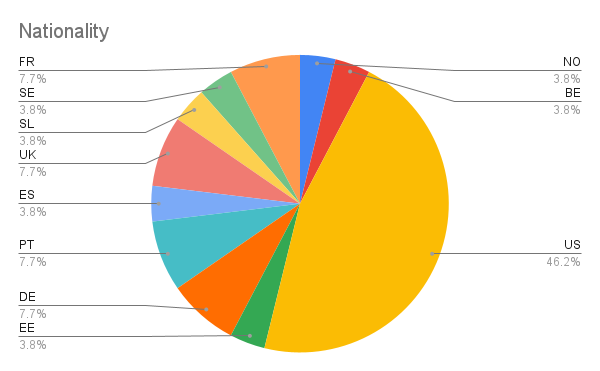
\includegraphics[scale=0.38]{fig/nationality.png}}
  \subfigure[]{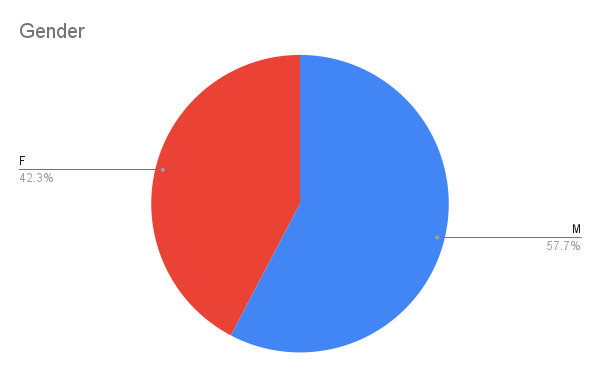
\includegraphics[scale=0.38]{fig/gender.png}}
  \caption{Nationality \& gender break up of participants for the
    \sympe.}
  \label{fig:country}
\end{figure}

We have shortlisted the following individuals as potential
participants in \symp with most who have confirmed participation. We
expect to invite a total of 27 scholars and along with 3 graduate
students for a total of $\sim 30$ participants, we believe will make
the symposium viable to achieve the goals we have set out for it. It
shows a broad dispersion of disciplines, relevant to ocean
observation, gender and geography. Given the constraints of the
symposium, including it being held while there is substantial
uncertainty in how the pandemic situation will evolve, we believe it
would be in the best interests to narrow the participation to
residents of the Americas and Europe. This is reflected in the detail
in Table \ref{tab:part}. % and is a starting point to pull together the
% actual participants.


\begin{table}[H]
  \footnotesize{
\begin{tabular}{|p{3.5cm}|p{0.7cm}|p{4.0cm}|p{0.5cm}|p{6.0cm}|}
% {lllll}
  \rowcolor{Gray}
  \bfseries Name& \bfseries M/F&\bfseries Institution & \bfseries Country& \bfseries Specialization\\
  Aida Alvera Az\'{a}rate*    & F   & Univ. of Leige                        & BE       & Remote Sensing, modeling                        \\
  \hline
  Jo Eidsvik*               & M   & NTNU                                  & NO       & Statistical Sampling                            \\
  \hline
  Kanna Rajan*              & M   & SIFT LLC/Univ. of Porto            & US       & AI, Autonomous systems           \\
  \hline
  Maarja Krusma            & F   & Tallinn Inst. of Tech                 & EE  & Sensors/robotics                                \\
  \hline
  Ralf Bachmeyer           & M   & Univ. of Bremen                       & DE       & Marine robotics, deep sea                       \\
  \hline
  Yogi Girdhar             & M   & Woods Hole                                  & US       & Marine robotics + ML                            \\
  \hline
  Ajit Subramaniam         & M   & Columbia University                        & US       & Bio-optics, Oceanography                        \\
  \hline
  Pere Ridao               & M   & Univ. of Girona& ES       & Grasping, robotics and control                            \\
  \hline
  Oliver Zelinsky          & M   & Univ. of Oldernburg                   & DE       & Instrumentation, sensors                        \\
  \hline
  Peter Girguis            & M   & Harvard University                               & US       & Genomics, micro-biology                         \\
  \hline
  Shubha Satyendernath     & F   & Plymouth Marine Labs                  & UK       & Remote Sensing, Ocean Color                     \\
  \hline
  Maha Haji                & F   & Cornell University                              & US       & Design optimization, Systems Engineering                   \\
  % \hline
  % Victoria Orphan          & F   & CalTech                               & US       & Microbial Ecology                               \\
  \hline
  Catarina Magalh\~aes      & F   & CIIMAR, Univ. of Porto                & PT       & Biological Oceanography                         \\
  \hline
  Rick Stumpf              & M   & NOAA                                  & US       & HABs, Ocean Optics                              \\
  \hline
  Jo\~ao Vitorino            & M   & Inst. Hidrografico                    & PT       & Physical Oceanography, modeling                    \\
  \hline
  Melissa Omand            & F   & Univ. of Rhode Island                 & US       & Physical Oceanography                              \\
  % \hline
  % Julien Brajard           & M   & Sorbonne / Nansen centre              & FR       & Data assimilation, machine learning             \\
  \hline
  Annalisa Bracco          & F   & Georgia Tech                          & US       & Ocean physics, meso-scale dynamics              \\
  % \hline
  % Marta Chantal Ribeiro    & F   & UN \& Univ. of Porto                  & PT       & Law of the Sea                                  \\
  \hline
  Geoff Hollinger          & M   & Oregon State Univ                     & US       & Robotics, Swarms, Sampling                              \\
  % \hline
  % Chelle Gentemann         & F   & Farallon Institute                    & US       & Remote Sensing (SST), air-sea fluxes \\
  \hline
  Ivona Cetini\'{c}            & F   & NASA Goddard                            & US       & Ocean colour, ocean biogeochemistry  \\
  \hline
  Matja\u{z} Li\u{c}er             & M   & National Inst. of Biology                                   & SL & Physical oceanography, ML, modelling            \\
  \hline
  Bastien Queste           & M   & U. Gothenburg                         & SE       & Oceanographer, AUVs\\                            
  \hline
  Allison Schaap           & F   & National Oceanography Center              & UK       & Micro-fluidics, ocean biogeochemistry, lab-on-a-chip\\
  \hline
  Lars Stemmann            & M & Sorbonne University                     & FR & Plankton ecology, biological pump, imaging systems\\
  \hline
  Sophie Clayton           & F   & Old Dominion University              & US       & Phytoplankton Ecology, Physical-Biological Interactions\\
  \hline
  Marina Levy              & F   & L'OCEAN                              & FR       & Ocean physics, biogeochemistry, plankton and marine ecosystems\\
  \hline
  Pierre Lermusiaux        & M   & MIT & US       &Modeling, assimilation \& prediction\\
  \hline
  Jo\~ao Sousa               & M   & Univ. of Porto & PT       &
                                                                 Control systems \& marine robotics                      \\
  \hline
\end{tabular}
}
\caption{Confirmed participants (including organizers) for the
  \sympe. * == organizer.}
\label{tab:part}
\end{table}

